% !TeX spellcheck = en_US
% !TeX encoding = utf8
% !TeX program = pdflatex

% \pdfminorversion=4
\documentclass[	%10pt
				% ,handout
				% ,notes=show
				% ,draft
				]{beamer}


\usepackage[T1]{fontenc}
\usepackage{rubfonts2009}
\usepackage{import}
\usetheme[alternativetitlepage=normal]{Rub}
% \usetheme{Berlin}
\usepackage{bm}
% \usetheme{Warsaw}
% \usecolortheme{seahorse}
% \usecolortheme{rose}
% \usefonttheme[onlylarge]{structuresmallcapsserif}
% \usefonttheme[onlysmall]{structurebold}
\setbeamercovered{transparent}
\usepackage{pgfplots}
\usepackage{intcalc}
\usepackage{graphicx}
\usepackage{amsmath}
\usepackage{array}
\usepackage{amssymb}
\usepackage{pgfplotstable}
\usepackage{caption}
\usepackage[
%disable
]{todonotes}
\usepackage[final]{pdfpages}
\usepackage{etoolbox}
\usepackage[backend=bibtex]{biblatex}
\usepackage[autostyle=true]{csquotes}

%broken biblatex http://tex.stackexchange.com/questions/311426/bibliography-error-use-of-blxbblverbaddi-doesnt-match-its-definition-ve
\makeatletter
\def\blx@maxline{77}
\makeatother

\usepackage{multirow}
%\captionsetup[figure]{name=} % dunno what this is, but it generates a warning so i comment it out

% \setbeamercolor{title}{fg=red!80!black}


\usepackage[english]{babel}
\usepackage[utf8]{inputenc}
\usetikzlibrary{shapes, arrows.meta, positioning, decorations.pathmorphing, math, calc, fit, chains, matrix, decorations.pathreplacing, trees, backgrounds, tikzmark, decorations.markings}

\usepackage{xcolor}
% \usepackage[table]{xcolor}
\PassOptionsToPackage{table}{xcolor}
% \usepackage{tabularx}
% \usepackage{mathptmx,amsmath}
\usepackage{graphicx}
\addbibresource{../database.bib}
\linespread{1.3} % increase baselineskip (spacing between lines)
\title{Design and Implementation of an LDPC-based FEC encoder/decoder suitable for Storage devices}
% \subtitle[]{}
\author[Henry Bathke]{Henry Bathke}
\institute[RUB-ESIT]{Ruhr University of Bochum \linebreak Chair for Embedded Systems for Information Technology}
\date{15. March 2018}
\usetikzlibrary{shapes, arrows.meta, positioning, decorations.pathmorphing, math, calc}
\setbeamercolor{framesubtitle}{fg=gelbgruen}

\pgfplotscreateplotcyclelist{hollow}{%
	mark=o,color=red,thick\\%
	mark=square,color=brown,thick\\%
	mark=x,color=green!50!black,thick\\%
	mark=triangle,color=blue,thick\\%
	mark=diamond,color=black,thick\\%
}



\AtBeginSection[]
{
  \begin{frame}[noframenumbering]
    \tableofcontents[currentsection, currentsubsection]
    \frametitle{Outline}
  \end{frame}
}
\AtBeginSubsection[]
{
  \begin{frame}[noframenumbering]
    \frametitle{Outline}
    \tableofcontents[currentsection,currentsubsection]
  \end{frame}
}


\DeclareMathOperator{\sign}{sign}
\DeclareMathOperator*{\argmin}{arg\,min}
\graphicspath{ {image/} }

\setbeamercovered{invisible}
%%%%%%%%%%%%%%%%%%%%%%%%%%%%%%%     Title Page     %%%%%%%%%%%%%%%%%%%%%%%%%%%%%%%%%%%
\pgfplotsset{compat=1.15}
\begin{document}
	
\begin{frame}[plain]
  \titlepage
\end{frame}

%%%%%%%%%%%%%%%%%%%%%%%%%%%%%%%     Outline     %%%%%%%%%%%%%%%%%%%%%%%%%%%%%%%%%%%
\begin{frame}
  \frametitle{Outline}
  % \tableofcontents[pausesections]
  % \tableofcontents[hideallsubsections]
  \tableofcontents
\end{frame}

%%%%%%%%%%%%%%%%%%%%%%%%%%%%%%%     Motivation     %%%%%%%%%%%%%%%%%%%%%%%%%%%%%%%%%%%
\section{Motivation}
\begin{frame}
	\frametitle{Motivation}
	\begin{itemize}
		\item Build a Hardware encoder and decoder suitable for storage devices
		\item Create a system for testing the encoder and decoder
	\end{itemize}

\end{frame}

%%%%%%%%%%%%%%%%%%%%%%%%%%%%%%%     Basics     %%%%%%%%%%%%%%%%%%%%%%%%%%%%%%%%%%%
\section{LDPC Codes}
\begin{frame}[fragile]
	\frametitle{Low Density Parity Check (LDPC) Codes}
	\begin{itemize}
		\item Multiple parity check equations
		\item Each bit is contained in multiple equations
		\item With these equations we can correct errors
		\item <2-> We construct the check matrix with the check equations
	\end{itemize}
	\visible<2->{
		\begin{align*}
			& \tikzmark{x1}x_1 \oplus \tikzmark{x2}x_3 \oplus \tikzmark{x3}x_4 \oplus \tikzmark{x4}x_7 = 0 \\
			\\
			\bm{H} = & \left[\begin{matrix}
				0 & \tikzmark{m1}1 & 0 & \tikzmark{m2}1 & \tikzmark{m3}1 & 0 & 0 & \tikzmark{m4}1 \\ 
				1 & 1 & 1 & 0 & 0 & 1 & 0 & 0 \\
				0 & 0 & 1 & 0 & 0 & 1 & 1 & 1 \\
				1 & 0 & 0 & 1 & 1 & 0 & 1 & 0
		\end{matrix}\right]	
		\end{align*}
		
		\begin{tikzpicture}[remember picture,overlay]
			%\draw[->] 
			\draw[->] ([shift={(1ex,-1ex)}]pic cs:x1) -- ([shift={(1pt,1em)}]pic cs:m1);
			\draw[->] ([shift={(1ex,-1ex)}]pic cs:x2) -- ([shift={(1pt,1em)}]pic cs:m2);
			\draw[->] ([shift={(1ex,-1ex)}]pic cs:x3) -- ([shift={(1pt,1em)}]pic cs:m3);
			\draw[->] ([shift={(1ex,-1ex)}]pic cs:x4) -- ([shift={(1pt,1em)}]pic cs:m4);
		\end{tikzpicture}
	}
\end{frame}

\begin{frame}
	\frametitle{Quasi Cyclic Low Density Parity Check (LDPC)}
	\begin{itemize}
		\item High complexity of LDPC codes
		\item Reduce complexity by adding structure to the PCM
		\item Split PCM into submatrices
		\item Only allow shifted version of a submatrix
	\end{itemize}
	\begin{equation*}
		\bm{B} = \left[\begin{matrix}
			-1 & 0 & 2 & -1\\
			0 & 1 & -1 & -1\\
			-1 & 1 & 0 & 2\\
		\end{matrix}\right]
	\end{equation*}
\end{frame}

%%%%%%%%%%%%%%%%%%%%%%%%%%%%%%%     Approach     %%%%%%%%%%%%%%%%%%%%%%%%%%%%%%%%%%%

\begin{frame}[fragile]
	\frametitle{Encoding}
	\begin{itemize}
		\item Is usually done with generator matrix
		\item The generator matrix is dense due to the inversion
		\item With long codes the dense matrix multiplication is large
		\item Use transforms on the PCM to convert it into a more desireable form\cite{QiGo07}
	\end{itemize}
	
\end{frame}

\begin{frame}[fragile]
	\frametitle{Encoding}
	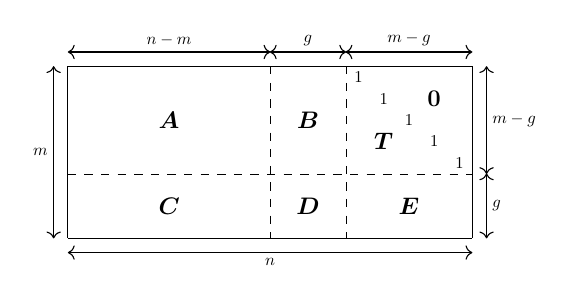
\begin{tikzpicture}[
		style1/.style={
				matrix of math nodes,
				every node/.append style={text width=#1,align=center,minimum height=3ex},
				nodes in empty cells,
			},
			scale=0.6,
			every node/.style={scale=0.6}
		]
		\matrix[style1=0.3cm] (1mat) {
			& & & & & & & & & & & & & & & \\
			& & & & & & & & & & & & & & & \\
			& & & & & & & & & & & & & & & \\
			& & & & & & & & & & & & & & & \\
			& & & & & & & & & & & & & & & \\
			& & & & & & & & & & & & & & & \\
			& & & & & & & & & & & & & & & \\
			& & & & & & & & & & & & & & & \\
		};
		\draw[dashed] (1mat-5-1.south west) -- (1mat-5-16.south east);
		\draw[dashed] (1mat-1-11.north east) -- (1mat-8-11.south east);
		\draw[dashed] (1mat-1-8.north east) -- (1mat-8-8.south east);

		\node [font=\Large] at ($(1mat-3-4)!0.5!(1mat-3-5)$) {$\bm{A}$};
		\node [font=\Large] at (1mat-3-10) {$\bm{B}$};

		\node [font=\Large] at (1mat-4-13) {$\bm{T}$};
		\node [font=\Large] at (1mat-2-15) {$\bm{0}$};

		\node [font=\Large] at ($(1mat-7-4)!0.5!(1mat-7-5)$) {$\bm{C}$};
		\node [font=\Large] at (1mat-7-10) {$\bm{D}$};
		\node [font=\Large] at (1mat-7-14) {$\bm{E}$};

		\node at (1mat-1-12) {1};
		\node at (1mat-2-13) {1};
		\node at (1mat-3-14) {1};
		\node at (1mat-4-15) {1};
		\node at (1mat-5-16) {1};
		
		\draw (1mat-1-1.north west) -- (1mat-8-1.south west);
		\draw (1mat-1-16.north east) -- (1mat-8-16.south east);
		\draw (1mat-1-1.north west) -- (1mat-1-16.north east);
		\draw (1mat-8-1.south west) -- (1mat-8-16.south east);

		\draw [<->] ([yshift=-3mm]1mat-8-1.south west) -- node[below] {$n$} ([yshift=-3mm]1mat-8-16.south east);
		\draw [<->] ([xshift=-3mm]1mat-1-1.north west) -- node[left] {$m$} ([xshift=-3mm]1mat-8-1.south west);

		\draw [<->] ([yshift=3mm]1mat-1-1.north west) -- node[above] {$n-m$} ([yshift=3mm]1mat-1-8.north east);
		\draw [<->] ([yshift=3mm]1mat-1-9.north west) -- node[above] {$g$} ([yshift=3mm]1mat-1-11.north east);
		\draw [<->] ([yshift=3mm]1mat-1-12.north west) -- node[above] {$m-g$} ([yshift=3mm]1mat-1-16.north east);

		\draw [<->] ([xshift=3mm]1mat-1-16.north east) -- node[right] {$m-g$} ([xshift=3mm]1mat-5-16.south east);
		\draw [<->] ([xshift=3mm]1mat-6-16.north east) -- node[right] {$g$} ([xshift=3mm]1mat-8-16.south east);
	\end{tikzpicture}
	\begin{itemize}
		\item Reach minimum gap $g$ by doing only row and column permutations
		\item Only need an inverted matrix of size $g \times g$
	\end{itemize}
\end{frame}


\section{Encoding}
\begin{frame}
	\frametitle{Encoding}
	\begin{itemize}
		\item Only large sparse matrix multiplication and back substitution
		\item One small dense matrix multiplication
	\end{itemize}
	\begin{tabular}{l l}
		Operation & Type \\ \toprule
		$\bm{A}s^T$ & sparse multiplication \\
		$\bm{T}^{-1}\bm{A}s^T$ & sparse back substitution \\
		$-\bm{E}\bm{T}^{-1}\bm{A}s^T$ & sparse multiplication \\
		$\bm{C}s^T$ & sparse multiplication \\
		$\left(-\bm{E}\bm{T}^{-1}\bm{A}s^T\right) + \left(\bm{C}s^T\right)$ & vector addition \\
		$\bm{\phi}^{-1}\left(-\bm{E}\bm{T}^{-1}\bm{A}s^T + \bm{C}s^T\right)$ & dense $g\times g$ multiplication\\
	\end{tabular}
\end{frame}



\begin{frame}
	\frametitle{Encoding Hardware}
	\begin{itemize}
		\item Implemented as combinatorial logic
		\item Connects to the other modules with an axi stream bus
		\item Repacking is needed as bit counts dont evenly divide
		\item Encoder is generated from the QC PCM with Python scripts
	\end{itemize}
	For wifi ldpc with rate 0.5 it looks like this
	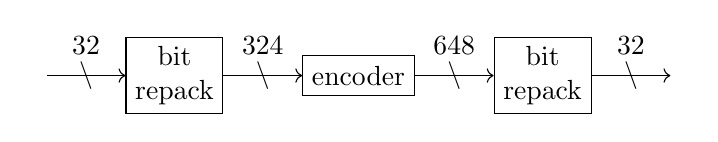
\begin{tikzpicture}[
		int/.style={draw,rectangle,node distance=.5cm,align=center,minimum width=.5cm, minimum height=.5cm},
		bitw/.style={decoration={markings,mark=at position 0.5 with{\node[transform shape] (tempnode) {$\backslash$};}},postaction={decorate}}
		]
		\node (rp1) [int] {bit\\repack};
		\node (enc) [right=of rp1,int] {encoder};
		\node (rp2) [right=of enc,int] {bit\\repack};
		\node (in) [left=of rp1] {};
		\node (out) [right=of rp2] {};
		\draw [->,bitw] (in) -- node[above=4pt] {32} (rp1);
		\draw [->,bitw] (rp1) -- node[above=4pt] {324} (enc);
		\draw [->,bitw] (enc) -- node[above=4pt] {648} (rp2);
		\draw [->,bitw] (rp2) -- node[above=4pt] {32} (out);
	
	\end{tikzpicture}
\end{frame}


\section{Decoding}
\begin{frame}
	\frametitle{Decoding}
	\begin{itemize}
		\item I implemented a message passing decoder
		\item Messages are passed along the edges on the tanner graph\cite{Ta81}
		\item Computations are done on the nodes
	\end{itemize}
	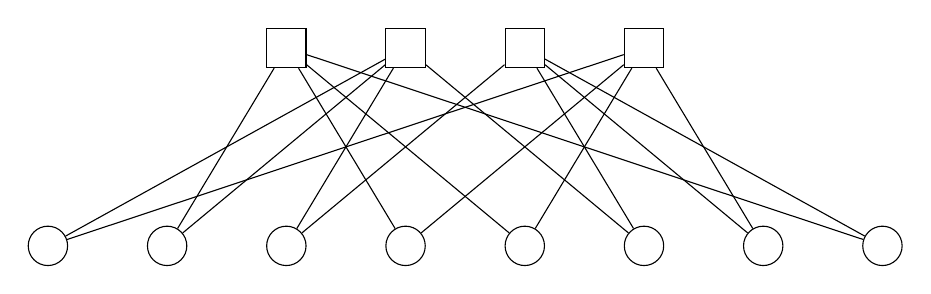
\begin{tikzpicture}[
		cnode/.style={draw,rectangle,node distance=1cm,align=center,minimum width=.5cm, minimum height=.5cm},
		vnode/.style={draw,circle,node distance=1cm,align=center,minimum width=.5cm, minimum height=.5cm}
	]
	\begin{scope}[start chain=going right, node distance=15mm]
		\node [vnode, on chain] (v0) {};
		\node [vnode, on chain] (v1) {};
		\node [vnode, on chain] (v2) {};
		\node [vnode, on chain] (v3) {};
		\node [vnode, on chain] (v4) {};
		\node [vnode, on chain] (v5) {};
		\node [vnode, on chain] (v6) {};
		\node [vnode, on chain] (v7) {};
	\end{scope}
	\begin{scope}[start chain=going right, node distance=15mm]
		\node [cnode, on chain, above=2cm of v2] (c0) {};
		\node [cnode, on chain] (c1) {};
		\node [cnode, on chain] (c2) {};
		\node [cnode, on chain] (c3) {};
	\end{scope}
	\draw (c0) -- (v1);
	\draw (c0) -- (v3);
	\draw (c0) -- (v4);	
	\draw (c0) -- (v7);
	\draw (c1) -- (v0);
	\draw (c1) -- (v1);
	\draw (c1) -- (v2);
	\draw (c1) -- (v5);
	\draw (c2) -- (v2);
	\draw (c2) -- (v5);
	\draw (c2) -- (v6);
	\draw (c2) -- (v7);
	\draw (c3) -- (v0);
	\draw (c3) -- (v3);
	\draw (c3) -- (v4);
	\draw (c3) -- (v6);
	\end{tikzpicture}
\end{frame}

\begin{frame}[fragile]
	\frametitle{Decoding}
	\begin{align*}
		r_{mn} & = \left( \prod_{n' \in M(m) \setminus n}\sign(q_{n'm}) \right) \min_{n' \in M(m) \setminus n}(\left|q_{n'm}\right|) \\
		q_{nm} & = y_n + \sum_{m' \in N(n) \setminus m}r_{m'n} \\
		L_n & = y_n + \sum_{m \in N(n)}r_{m'n}
	\end{align*}
	\begin{itemize}
		\item We have to implement these equations
		\item Can exploit similarities
	\end{itemize}
\end{frame}

\begin{frame}
	\frametitle{Hardware Decoding}
	\begin{itemize}
		\item two pass algorithm
		\item intermediate values stored im memory
	\end{itemize}
	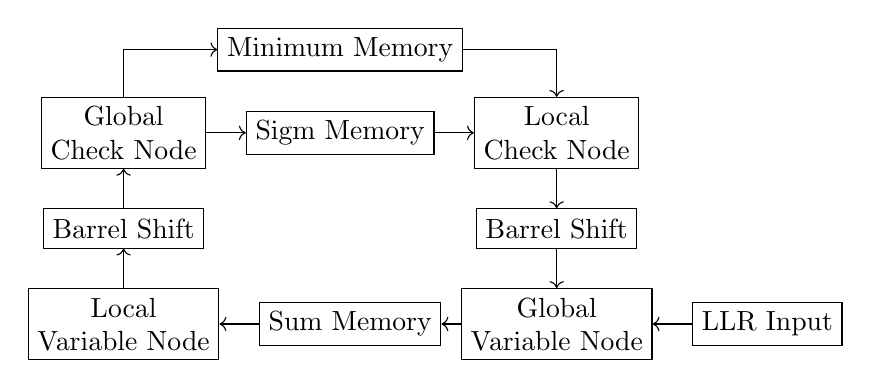
\begin{tikzpicture}[
		elem/.style={draw,rectangle,node distance=0.5cm,align=center,minimum width=.5cm, minimum height=.5cm}
	]
		\node (mime) [elem] {Minimum Memory};
		\node (sime) [elem,below=of mime] {Sigm Memory};
		\node (cngl) [elem,left=of sime] {Global\\Check Node};
		\node (rot1) [elem,below=of cngl] {Barrel Shift};
		\node (vnlo) [elem,below=of rot1] {Local\\Variable Node};
		\node (sume) [elem,right=of vnlo] {Sum Memory};
		\node (cnlo) [elem,right=of sime] {Local\\Check Node};
		\node (rot2) [elem,below=of cnlo] {Barrel Shift};
		\node (vngl) [elem,below=of rot2] {Global\\Variable Node};
		\node (llri) [elem,right=of vngl] {LLR Input};
	
		\draw [->] (mime) -| (cnlo);
		\draw [->] (sime) -- (cnlo);
		\draw [->] (cnlo) -- (rot2);
		\draw [->] (rot2) -- (vngl);
		\draw [->] (llri) -- (vngl);
		\draw [->] (vngl) -- (sume);
		\draw [->] (sume) -- (vnlo);
		\draw [->] (vnlo) -- (rot1);
		\draw [->] (rot1) -- (cngl);
		\draw [->] (cngl) |- (mime);
		\draw [->] (cngl) -- (sime);
	\end{tikzpicture}
	\centering
\end{frame}
\begin{frame}
	\frametitle{Hardware Decoding}
	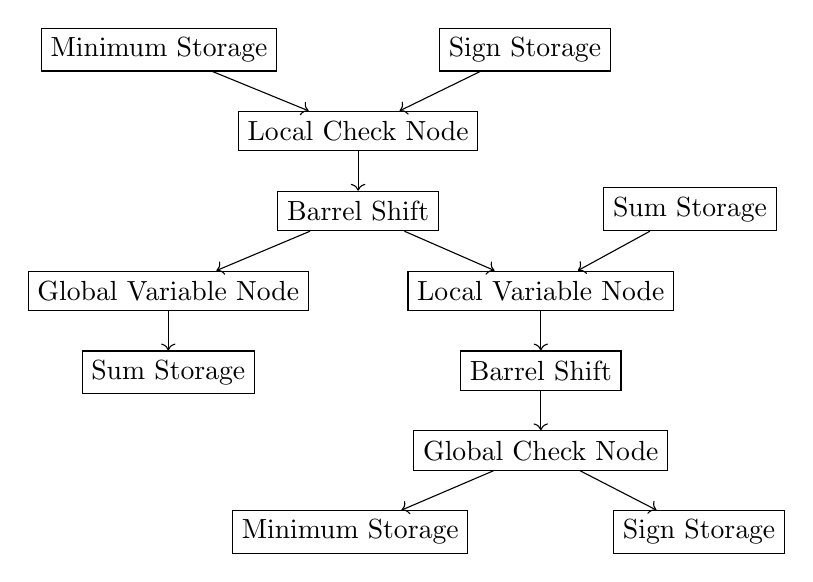
\begin{tikzpicture}
		[
	elem/.style={draw,rectangle,node distance=0.5cm,align=center,minimum width=.5cm, minimum height=.5cm}
	]
		\node (cnlo) [elem] {Local Check Node};
		\node (rol1) [elem,below=of cnlo] {Barrel Shift};
		\visible<1,3> {
			\node (vngl) [elem,below left=0.5cm and -0.4cm of rol1] {Global Variable Node};
			\node (sumr) [elem,below=of vngl] {Sum Storage};
		}
		\visible<2-3> {
			\node (vnlo) [elem,below right=0.5cm and -0.4cm of rol1] {Local Variable Node};
			\node (rol2) [elem,below=of vnlo] {Barrel Shift};
			\node (cngl) [elem,below=of rol2] {Global Check Node};

			\node (sums) [elem,above right=0.5cm and -0.9cm of vnlo] {Sum Storage};
			\node (minr) [elem,below left=0.5 and -0.7cm of cngl] {Minimum Storage};
			\node (sigr) [elem,below right=0.5cm and -0.7cm of cngl] {Sign Storage};
		}

		\node (mins) [elem,above left=0.5cm and -0.5cm of cnlo] {Minimum Storage};
		\node (sigs) [elem,above right=0.5cm and -0.5cm of cnlo] {Sign Storage};
		
		\draw [->] (mins) -- (cnlo);
		\draw [->] (sigs) -- (cnlo);
		\draw [->] (cnlo) -- (rol1);
		\visible<1,3> {
			\draw [->] (rol1) -- (vngl);
			\draw [->] (vngl) -- (sumr);
		}
	
		\visible<2-3> {
			\draw [->] (sums) -- (vnlo);
			\draw [->] (rol1) -- (vnlo);
			\draw [->] (vnlo) -- (rol2);
			\draw [->] (rol2) -- (cngl);
			\draw [->] (cngl) -- (minr);
			\draw [->] (cngl) -- (sigr);
		}
	\end{tikzpicture}
	\centering
\end{frame}

\begin{frame}[fragile]
	\frametitle{Hardware Decoding}
	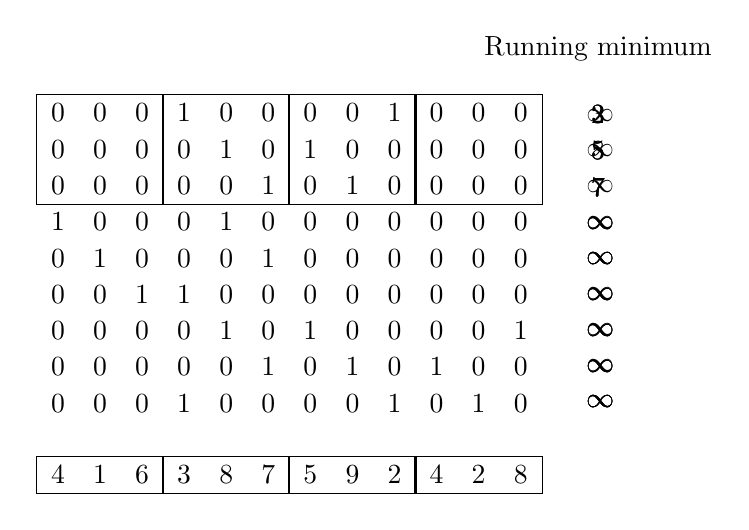
\begin{tikzpicture}[
		style1/.style={
				matrix of math nodes,
				every node/.append style={text width=#1,align=center,minimum height=3ex},
				nodes in empty cells,
			},
			scale=1.0,
			every node/.style={scale=1.0}
		]
		\matrix[style1=0.3cm] (1mat) {
			0 & 0 & 0 & 1 & 0 & 0 & 0 & 0 & 1 & 0 & 0 & 0 \\
			0 & 0 & 0 & 0 & 1 & 0 & 1 & 0 & 0 & 0 & 0 & 0 \\
			0 & 0 & 0 & 0 & 0 & 1 & 0 & 1 & 0 & 0 & 0 & 0 \\
			1 & 0 & 0 & 0 & 1 & 0 & 0 & 0 & 0 & 0 & 0 & 0 \\
			0 & 1 & 0 & 0 & 0 & 1 & 0 & 0 & 0 & 0 & 0 & 0 \\
			0 & 0 & 1 & 1 & 0 & 0 & 0 & 0 & 0 & 0 & 0 & 0 \\
			0 & 0 & 0 & 0 & 1 & 0 & 1 & 0 & 0 & 0 & 0 & 1 \\
			0 & 0 & 0 & 0 & 0 & 1 & 0 & 1 & 0 & 1 & 0 & 0 \\
			0 & 0 & 0 & 1 & 0 & 0 & 0 & 0 & 1 & 0 & 1 & 0 \\
		};
		\matrix[style1=0.3cm,below=0.2cm of 1mat] (2mat) {
			4 & 1 & 6 & 3 & 8 & 7 & 5 & 9 & 2 & 4 & 2 & 8 \\
		};
	
		
		\visible<1> {
			\draw (1mat-1-1.north west) rectangle (1mat-3-3.south east);
			\draw (2mat-1-1.north west) rectangle (2mat-1-3.south east);
			\matrix[style1=0.3cm,right=0.2cm of 1mat] (3mat) {
				\infty \\ \infty \\ \infty \\ \infty \\ \infty \\ \infty \\ \infty \\ \infty \\ \infty \\
			};
		}
		\visible<2> {
			\draw (1mat-1-4.north west) rectangle (1mat-3-6.south east);
			\draw (2mat-1-4.north west) rectangle (2mat-1-6.south east);
			\matrix[style1=0.3cm,right=0.2cm of 1mat] (3mat) {
				3 \\ 8 \\ 7 \\ \infty \\ \infty \\ \infty \\ \infty \\ \infty \\ \infty \\
			};
		}
		
		\visible<3> {
			\draw (1mat-1-7.north west) rectangle (1mat-3-9.south east);
			\draw (2mat-1-7.north west) rectangle (2mat-1-9.south east);
			\matrix[style1=0.3cm,right=0.2cm of 1mat] (3mat) {
				2 \\ 5 \\ 7 \\ \infty \\ \infty \\ \infty \\ \infty \\ \infty \\ \infty \\
			};
		}

		\visible<4> {
			\draw (1mat-1-10.north west) rectangle (1mat-3-12.south east);
			\draw (2mat-1-10.north west) rectangle (2mat-1-12.south east);
			\matrix[style1=0.3cm,right=0.2cm of 1mat] (3mat) {
				2 \\ 5 \\ 7 \\ \infty \\ \infty \\ \infty \\ \infty \\ \infty \\ \infty \\
			};
		}
	
		\node [above=0.2cm of 3mat] {Running minimum};
	\end{tikzpicture}
	\centering
\end{frame}


\section{Performance}
\begin{frame}
	\frametitle{Performance Testing}
	\begin{itemize}
		\item Used a ZedBoard
		\item Testing requires an encoder, channel, decoder setup
		\item AWGN channel
		\item Whole performance test is implemented on Hardware
		\item ARM cpu calculates test parameters and reads the error counts
	\end{itemize}
	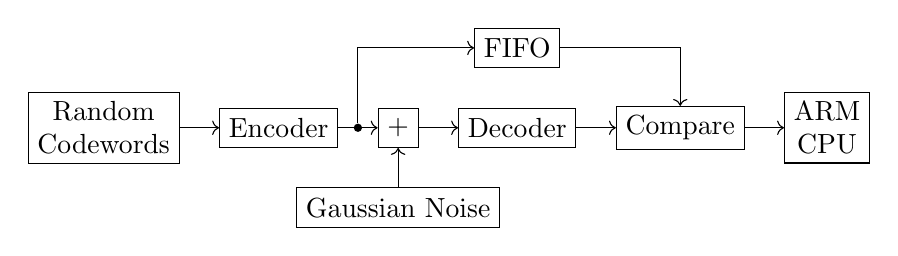
\begin{tikzpicture}
		[
	elem/.style={draw,rectangle,node distance=0.5cm,align=center,minimum width=.5cm, minimum height=.5cm},
	branch/.style={fill,shape=circle,minimum size=3pt,inner sep=0pt}
	]
		\node (rdi) [elem] {Random\\Codewords};
		\node (enc) [elem,right=of rdi] {Encoder};
		\node (add) [elem,right=of enc] {+};
		\node (dec) [elem,right=of add] {Decoder};
		\node (com) [elem,right=of dec] {Compare};
		\node (ran) [elem,below=of add] {Gaussian Noise};
		\node (fif) [elem,above=of dec] {FIFO};
		\node (arm) [elem,right=of com] {ARM\\CPU};
	
		\draw [->] (rdi) -- (enc);
		\draw [->] (enc) -- node[pos=0.5,branch] (test) {} (add);
		\draw [->] (add) -- (dec);
		\draw [->] (dec) -- (com);
		\draw [->] (ran) -- (add);
		\draw [->] (test) |- (fif);
		\draw [->] (fif) -| (com);
		\draw [->] (com) -- (arm);
	\end{tikzpicture}
\end{frame}

\section{Results}
\newcommand{\addgraph}[2]{\addplot table [col sep=tab,x index={0}, y index={#2}] {#1};
	\pgfplotstablegetcolumnnamebyindex{#2}\of{#1}\to{\colname}
	\addlegendentryexpanded{\colname}}
\pgfplotstableread[col sep=tab]{../data/sw_err_simple.dat}\basesim
\begin{frame}
	\frametitle{Simulation Results}
	802.11n LDPC code with rate 0.5
	\begin{tikzpicture}
		\begin{semilogyaxis}[width=11cm,height=\axisdefaultheight-10mm,xlabel={$E_b / N_0$} in dB, ylabel={Error Rate}, legend pos=south west]
			
			\only<1> {
				\addgraph{\basesim}{1}
				\addgraph{\basesim}{3}
			}

			\addgraph{\basesim}{2}
			\addgraph{\basesim}{4}
			\only<2> {
				\addgraph{\basesim}{6}
				\addgraph{\basesim}{7}
			}

		\end{semilogyaxis}
	\end{tikzpicture}
\end{frame}


\newcommand{\cleanaddgraph}[2]{\addplot table [mark=none,col sep=tab,x index={0}, y index={#2}] {#1};
	\pgfplotstablegetcolumnnamebyindex{#2}\of{#1}\to{\colname}
	\addlegendentryexpanded{\colname}
}

\begin{frame}
	\frametitle{Hardware Results}
	\begin{itemize}
		\item Decoder expects LLR
		\item Convert channel output to LLR
	\end{itemize}
	\begin{tikzpicture}[
		elem/.style={draw,rectangle,node distance=1cm,align=center,minimum width=.5cm, minimum height=.5cm},
		circ/.style={draw,circle,node distance=1cm,align=center,minimum width=.5cm, minimum height=.5cm},
		branch/.style={fill,shape=circle,minimum size=3pt,inner sep=0pt}]
		\node (gvg) [elem] {GVG};
		\node (mul) [circ, right=of gvg] {$\times$};
		\node (sig) [right=of mul] {$\sigma$};
		\node (plu) [elem,above=of mul] {+};
		\node (mus) [circ,left=of plu] {$\times$};
		\node (fac) [above=of mus] {Scale};
		\node (cha) [left=of mus] {Encoded};
		\node (llr) [circ,right=of plu] {$\times$};
		\node (llv) [above=of llr] {$\frac{2}{\sigma^2}$};
		\node (dec) [right=of llr] {Decoder};
		\draw [->] (gvg) -- (mul);
		\draw [->] (sig) -- (mul);
		\draw [->] (mul) -- (plu);
		\draw [->] (plu) -- (llr);
		\draw [->] (llv) -- (llr);
		\draw [->] (llr) -- (dec);
		\draw [->] (cha) -- (mus);
		\draw [->] (fac) -- (mus);
		\draw [->] (mus) -- (plu); 
	\end{tikzpicture}
	\centering
\end{frame}


\begin{frame}
	\frametitle{Hardware Results}
	Optimize the input scaling
	\begin{tikzpicture}
		\begin{semilogyaxis}[width=11cm,height=\axisdefaultheight-10mm,xlabel={$E_b / N_0$} in dB, ylabel={Error Rate}, legend pos=south west]
			\pgfplotstableread[col sep=tab]{../data/hw_opt_bit_val_coarse.dat}\hwoptbitbal
			\foreach \x in {1,...,7} {
				\cleanaddgraph{\hwoptbitbal}{\x};
			}
		\end{semilogyaxis}
	\end{tikzpicture}
\end{frame}

\begin{frame}
	\frametitle{Hardware Results}
	I chose a scaling of 0.75
	\begin{tikzpicture}
		\begin{semilogyaxis}[width=11cm,height=\axisdefaultheight-10mm,xlabel={$E_b / N_0$} in dB, ylabel={Error Rate}, legend pos=south west]
			\pgfplotstableread[col sep=tab]{../data/hw_opt_bit_val_fine.dat}\hwoptbitbal
			\foreach \x in {2,4,...,17} {
				\cleanaddgraph{\hwoptbitbal}{\x};
			}
		\end{semilogyaxis}
	\end{tikzpicture}
\end{frame}

\begin{frame}
	\frametitle{Hardware Results}
	\framesubtitle{Normalized Min Sum}
	\begin{tikzpicture}
		\begin{semilogyaxis}[width=11cm,height=\axisdefaultheight,xlabel={$E_b / N_0$} in dB, ylabel={Error Rate}, legend pos=south west]
			\pgfplotstableread[col sep=tab]{../data/hw_opt_norm.dat}\hwoptnorm
			\addgraph{\basesim}{7}
			\foreach \x in {5,...,8} {
				\cleanaddgraph{\hwoptnorm}{\x};
			}
		\end{semilogyaxis}
	\end{tikzpicture}
\end{frame}
%%%%%%%%%%%%%%%%%%%%%%%%%%%%%%%     Conclusion     %%%%%%%%%%%%%%%%%%%%%%%%%%%%%%%%%%%
\section{Conclusion and Outlook}
\begin{frame}
	\frametitle{Conclusion and Outlook}
	{\Large Conclusion}
	\begin{itemize}
		\item LDPC codes can be implemented on hardware
		\item 
	\end{itemize}
	{\Large Outlook}
	\begin{itemize}
		\item Look at power consumption
		\item Optimize area utilization
	\end{itemize}
\end{frame}

\begin{frame}
	\frametitle{Questions?}
	\centering
	\Huge
	Questions?
\end{frame}

\begin{frame}[allowframebreaks]
	\frametitle{References}
	\linespread{1}
	\printbibliography
\end{frame}

\end{document}

